\documentclass{scrbook}
\usepackage{graphicx} % Required for inserting images
\usepackage{tabularx} % Required for fixed width tables
\usepackage{scrlayer-scrpage} % Required for the subtitles
\usepackage{url} % Required for the URLs
\usepackage{hyperref} % Required for the URLs
\usepackage{listings} % Required for the code snippets

% Put the caption of the snippets at the bottom
\lstset{
    captionpos=b
}


\title{CSS: Cascaded Style Sheet}
\subtitle{Ambient intelligence course (A.Y. 2025/2026)\\Topic taught by Prof. Floriano Scioscia}
\author{Gabriele Colapinto}
\date{\today}

\begin{document}

\maketitle
\thispagestyle{empty}

{\Large\textbf{License}} \\
{Notes from Ambient intelligence (A.Y. 2025/2026) by Gabriele Colapinto. 
Course taught by professors Michele Ruta, Floriano Scioscia, Arnaldo Tomasino, Davide Loconte — 
Licensed under CC BY-NC 4.0.\\
\url{https://creativecommons.org/licenses/by-nc/4.0/}}

\vspace*{\fill}
\rule{\textwidth}{0.2pt}
\small{© 2025 Gabriele Colapinto \\
Released under the \href{https://creativecommons.org/licenses/by-nc/4.0/}{Creative Commons Attribution–NonCommercial 4.0 International License}}

\clearpage

\tableofcontents

\chapter{Applying the Style: CSS Fundamentals}

\begin{figure}
    \centering
    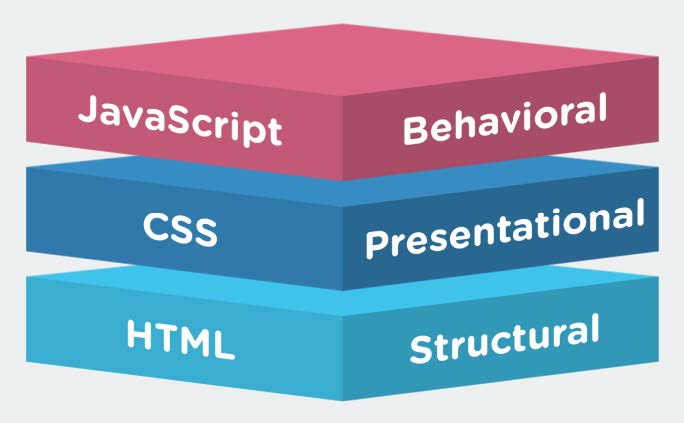
\includegraphics[width=0.5\linewidth]{Images/Web_page_stack.jpg}
    \caption{Web page stack}
    \label{fig:web_page_stack}
\end{figure}

CSS transforms a basic HTML structure into a polished and visually engaging user experience. It dictates everything from typography and color to layout and spacing. Understanding the core mechanics of CSS—its syntax, application methods, and the powerful selection system that connects styles to specific HTML elements—is essential for creating modern, well-designed websites.

\section{How CSS Works: The Cascade}

The "Cascading" in Cascading Style Sheets is a crucial concept. It refers to the ordered process by which styles are applied to a document. Rules that are read later in this process can override rules defined earlier, creating a waterfall-like flow of style inheritance and precedence. \\


There are three primary methods for inserting a style sheet into an HTML document:

\begin{enumerate}
    \item \textbf{External Style Sheet:} Styles are defined in a separate \texttt{.css} file and linked to the HTML document using the \texttt{<link>} tag within the \texttt{<head>} section. This is the industry best practice, as it cleanly separates content from presentation and allows a single file to style an entire website.
    \begin{lstlisting}[language=HTML, caption={Linking of an external style sheet}]
    <head>
        <link rel="stylesheet" type="text/css" href="mystyle.css">
    </head>
    \end{lstlisting}
    
    \item \textbf{Internal Style Sheet:} Styles are placed directly within the \texttt{<head>} section of an HTML document, inside a \texttt{<style>} tag. This method is useful for single-page styling but is less scalable than external sheets.
    \begin{lstlisting}[language=HTML, caption={Style sheet definition in the head tag}]
    <head>
        <style>
            h1 {
                color: blue;
            }
        </style>
    </head>
    \end{lstlisting}
    
    \item \textbf{Inline Style:} Styles are applied directly to a single HTML element using the \texttt{style} attribute. This approach mixes content with presentation and should be used sparingly, as it has the highest priority and can be difficult to override.
    \begin{lstlisting}[language=HTML, caption={Inline element style definition}]
    <h1 style="color: blue;">This is a heading.</h1>
    \end{lstlisting}
\end{enumerate}

The priority of these styles follows a specific cascading order, from lowest to highest (See figure ~\ref{fig:cascading_order}):

\begin{enumerate}
    \item \textbf{Browser default:} Every browser has its own default styles for HTML elements.
    \item \textbf{External and internal style sheets:} Styles defined in the document's \texttt{<head>}. If there are conflicting rules, the one that appears last takes precedence.
    \item \textbf{Inline style:} Styles applied directly to an element with the \texttt{style} attribute have the highest priority and will override rules from all other sources.
\end{enumerate}

\begin{figure}
    \centering
    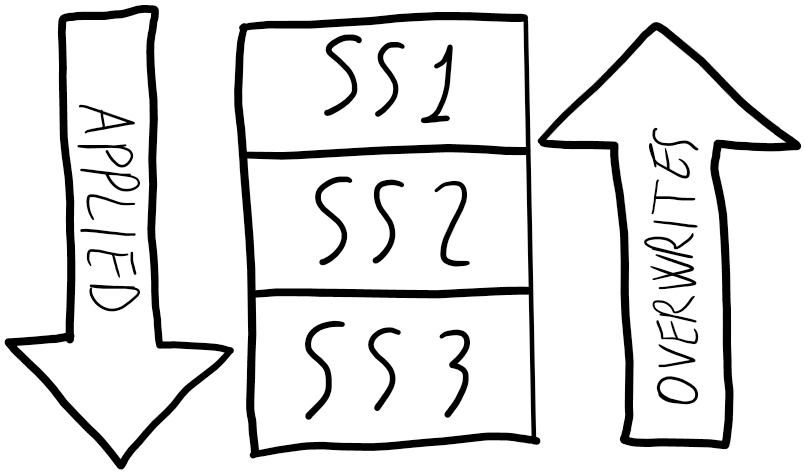
\includegraphics[width=0.5\linewidth]{Images/Cascading_order.png}
    \caption{CSS cascading order}
    \label{fig:cascading_order}
\end{figure}

\section{The Language of CSS: Rules, Selectors, and Properties}

\begin{figure}[htbp]
    \centering
    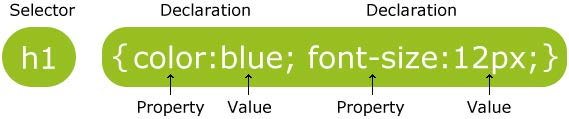
\includegraphics[width=\linewidth]{Images/CSS_syntax.jpg}
    \caption{CSS syntax}
    \label{fig:css_syntax}
\end{figure}

A CSS style sheet consists of a set of rules. Each rule has two main parts: a \textbf{selector} and a \textbf{declaration block} (See figure ~\ref{fig:css_syntax}). The selector points to the HTML element(s) you want to style, while the declaration block, enclosed in curly braces \texttt{\{\}}, contains one or more property-value pairs separated by semicolons. \\


CSS provides a rich set of selectors for targeting elements with precision:

\begin{itemize}
    \item \textbf{Basic Selectors}
    \begin{itemize}
        \item \texttt{element}: Selects all elements of a specific type (e.g., \texttt{p} selects all paragraphs).
        \item \texttt{id} (\texttt{\#id}): Selects the single element with a specific, unique \texttt{id} attribute.
        \item \texttt{class} (\texttt{.class}): Selects all elements that have a specific \texttt{class} attribute.
    \end{itemize}
    \item \textbf{Attribute Selector}
    \begin{itemize}
        \item \texttt{[attribute]}: Selects all elements that possess a given attribute (e.g., \texttt{p[name]} selects paragraphs with a \texttt{name} attribute).
    \end{itemize}
    \item \textbf{Proximity \& Combinator Selectors}
    \begin{itemize}
        \item \textbf{Descendant} (\texttt{div h1}): Selects all \texttt{<h1>} elements that are located anywhere inside a \texttt{<div>} element.
        \item \textbf{Direct Child} (\texttt{div > h1}): Selects only \texttt{<h1>} elements that are direct children of a \texttt{<div>}.
        \item \textbf{Adjacent Sibling} (\texttt{h1 + h2}): Selects an \texttt{<h2>} element that is placed immediately after an \texttt{<h1>} element at the same hierarchical level.
    \end{itemize}
    \item \textbf{Pseudo-class Selector}
    \begin{itemize}
        \item \texttt{a:hover}: Selects an element based on its current state, such as when a user hovers their mouse over a link.
    \end{itemize}
    \item \textbf{Pseudo-element Selector}
    \begin{itemize}
        \item \texttt{p::first-letter}: Selects and styles a specific part of an element, such as the first letter of a paragraph.
    \end{itemize}
    \item \textbf{Grouping \& Universal Selectors}
    \begin{itemize}
        \item \textbf{Grouping} (\texttt{h1, h2}): Applies the same style rules to multiple selectors by separating them with a comma.
        \item \textbf{Universal} (\texttt{*}): Selects every single element on the page.
    \end{itemize}
\end{itemize}

\section{Common Properties and Values}

CSS properties accept a wide variety of values, including units for size and multiple notations for color.

\subsection{Size Units}

\begin{itemize}
    \item \textbf{Absolute Units:} These are fixed and do not change based on other elements.
    \begin{itemize}
        \item \texttt{px}: Logical pixels, the most 
        common unit for screen-based design.
        
        \item \texttt{pt}: Typographic points (1pt = 1/72 of an inch), typically used for print media.

        \item \texttt{in}: Inches.
        \item \texttt{cm}
        \item \texttt{mm}
    \end{itemize}
    
    \item \textbf{Relative Units:} These are flexible and scale in relation to another value.
    \begin{itemize}
        \item \texttt{em}: Relative to the font-size of the element itself.
        \item \texttt{\%}: Relative to the size of the parent container element. (See figure ~\ref{fig:relative_width_example})
    \end{itemize}
\end{itemize}

\begin{figure}
    \centering
    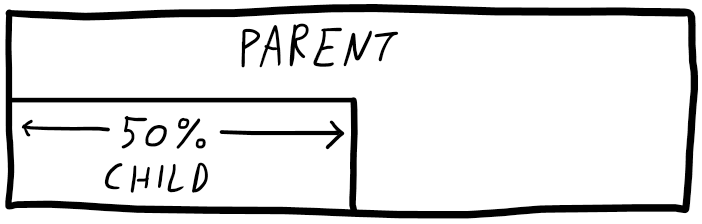
\includegraphics[width=\linewidth]{Images/Relative_width_example.png}
    \caption{An example of an element with a width equal to the 50\% of the width of the parent container element.}
    \label{fig:relative_width_example}
\end{figure}

\subsection{Color Values}

Color can be specified in several ways:

\begin{itemize}
    \item \textbf{Predefined Name:} Using a standard color name (e.g., \texttt{red}, \texttt{blue}).
    \item \textbf{RGB Function:} Using the \texttt{rgb()} function to specify values (0-255) for Red, Green, and Blue channels (e.g., \texttt{rgb(255, 0, 0)}).
    \item \textbf{Hexadecimal Notation:} A six-digit code preceded by a hash (\texttt{\#}) that represents the RGB values in hexadecimal format (e.g., \texttt{\#FF0000}). Each pair of characters corresponds to the Red, Green, and Blue values, where \texttt{FF} is equivalent to 255.
\end{itemize}

\subsection{Font family}

The \texttt{font-family} property is used to specify the typeface for text. It accepts a prioritized list of font names, known as a "font stack." The browser will attempt to use the first font in the list; if it is not available on the user's system, it will try the next one, and so on. It is a crucial best practice to end the list with a generic font family (e.g., \texttt{sans-serif} or \texttt{serif}) as a fallback to ensure the text is always rendered in a suitable style.

\chapter{The CSS Box Model: The Foundation of Layout}

\begin{figure}[htbp]
    \centering
    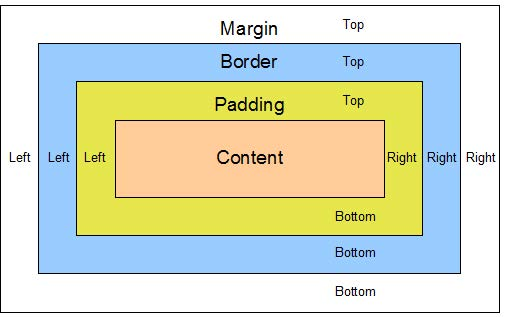
\includegraphics[width=0.5\linewidth]{Images/CSS_box_model.jpg}
    \caption{CSS box model}
    \label{fig:box_model}
\end{figure}

The CSS Box Model (figure ~\ref{fig:box_model}) is the fundamental concept governing how every visible HTML element is rendered as a rectangular area on a web page. When a browser displays a document, it assigns a box to each element, and understanding the components of this box is critical for controlling element dimensions, spacing, and overall page layout. Mastering the box model is the first step toward building predictable and well-structured designs. \\

The model is composed of four primary components, layered from the inside out:

\begin{itemize}
    \item \textbf{Content:} The innermost layer where the actual content of the element, such as text and images, appears.
    \item \textbf{Padding:} The transparent area surrounding the content, creating a buffer \textit{inside} the element's border.
    \item \textbf{Border:} A line that goes around the padding and content. Its appearance can be customized in terms of style, color, and thickness.
    \item \textbf{Margin:} The transparent area outside the border, creating space \textit{between} this element and any adjacent elements.
\end{itemize}

\section{Customizing the Border}

\begin{figure}
    \centering
    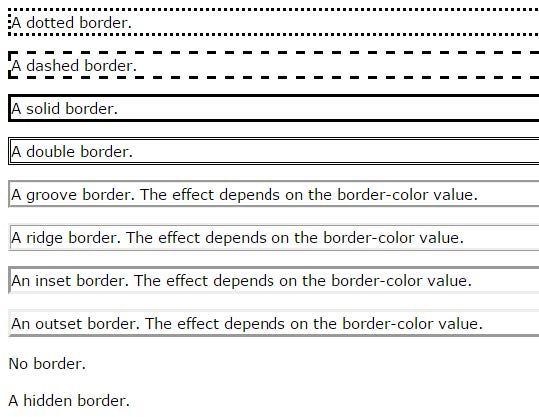
\includegraphics[width=\linewidth]{Images/Border_styles.jpg}
    \caption{Border styles}
    \label{fig:border_styles}
\end{figure}

The appearance of an element's border is specified by the \texttt{border-style} property (See figure ~\ref{fig:border_styles} and table ~\ref{tbl:border_style_values}). This property accepts a range of keyword values that define the visual style of the line drawn around the element's padding and content.

\begin{table}[h]
    \centering
    \begin{tabular}{|l|l|}
    \hline
    \textbf{Style Value} & \textbf{Description} \\
    \hline
    \texttt{dotted} & Defines a border composed of dots. \\
    \hline
    \texttt{dashed} & Defines a border composed of dashes. \\
    \hline
    \texttt{solid} & Defines a solid, single-line border. \\
    \hline
    \texttt{double} & Defines a double border. \\
    \hline
    \texttt{groove} & Defines a 3D grooved border. The effect depends on the border-color value. \\
    \hline
    \texttt{ridge} & Defines a 3D ridged border. The effect depends on the border-color value. \\
    \hline
    \texttt{inset} & Defines a 3D inset border, creating the appearance of being embedded. \\
    \hline
    \texttt{outset} & Defines a 3D outset border, creating the appearance of coming out. \\
    \hline
    \texttt{none} & Defines no border. \\
    \hline
    \texttt{hidden} & Defines a hidden border. \\
    \hline
    \end{tabular}
    \caption{Border Style Values}
    \label{tbl:border_style_values}
\end{table}

Once we understand how every element is represented as a box, we can explore how CSS allows us to precisely position these boxes on the page.

\chapter{Controlling Element Position and Stacking Order}

Beyond defining the space an element occupies, CSS provides powerful properties to control its exact placement on the page. You can position an element within the normal document flow, fix it relative to the browser's viewport, or place it relative to its parent or other ancestor elements. This level of control is essential for creating complex and interactive layouts.

\section{The Property}

The \texttt{position} property specifies the positioning method used for an element. It can take one of four primary values. \\

\subsection{static}

This is the default value. Elements are positioned according to the normal flow of the page. By default, block elements are stacked vertically, one after the other, while inline elements are aligned horizontally in a row.

\begin{lstlisting}
div.static { 
    position: static; 
}
\end{lstlisting}

\subsection{relative}

The element is positioned relative to its normal, static position in the document flow. You can then use the offset properties \texttt{left}, \texttt{top}, \texttt{bottom}, and \texttt{right} to move it away from that original spot without affecting the layout of surrounding elements.

\begin{lstlisting}
div.relative { 
    position: relative; 
    left: 30px; 
}
\end{lstlisting}

\subsection{fixed}

The element is positioned relative to the viewport (the browser window). It remains in the same place even when the page is scrolled. This is often used for persistent user interface elements like navigation bars, cookie policy banners, or chatbot buttons that should always be accessible.

\begin{lstlisting}
div.fixed { 
    position: fixed; 
    bottom: 0; 
    right: 0; 
    width: 300px; 
}
\end{lstlisting}

\subsection{absolute}

The element is positioned relative to its nearest positioned ancestor (i.e., the closest parent element that has a \texttt{position} value other than \texttt{static}). If no such ancestor exists, the element is positioned relative to the initial containing block, which is the \textbf{viewport}.

\begin{lstlisting}
div.absolute { 
    position: absolute; 
    top: 80px; 
    right: 0; 
    width: 200px; 
    height: 100px; 
}
\end{lstlisting}

\section{Managing overlapping elements}

When you manually control element positions, it's possible for their boxes to overlap. The \texttt{z-index} property specifies the stack order of these overlapping elements, determining which one appears on top. An element's \texttt{z-index} can be a positive or negative integer, with a default value of \texttt{0}. \\

The stacking order is determined by two simple rules:

\begin{enumerate}
    \item An element with a greater \texttt{z-index} value is always rendered in front of an element with a lower value.
    \item If two overlapping elements have the same \texttt{z-index}, the one that appears last in the HTML code is rendered on top of the other.
\end{enumerate}

While manual positioning provides fine-grained control, modern web development often requires layouts that adapt automatically to different devices and screen sizes, which leads to the principles of Responsive Web Design.

\chapter{An Introduction to Responsive Web Design (RWD)}

\begin{figure}[htbp]
    \centering
    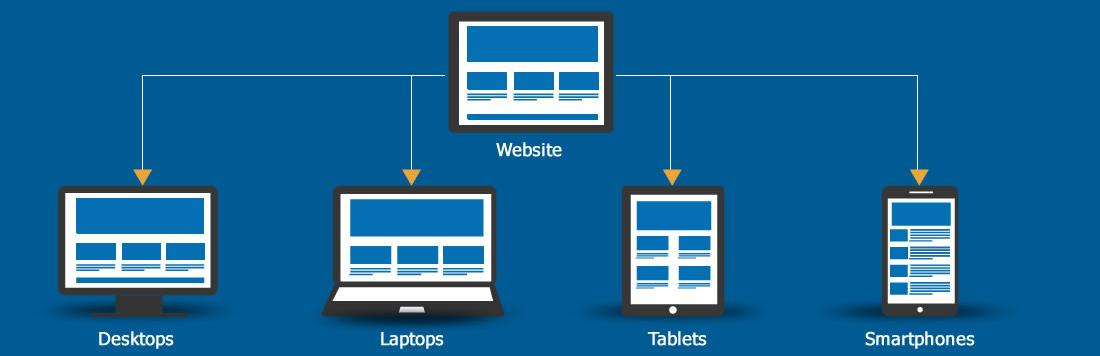
\includegraphics[width=\linewidth]{Images/Responsive_web_design.jpg}
    \caption{Responsive Web Design}
    \label{fig:rwd}
\end{figure}

Responsive Web Design (RWD) is a design approach that uses only HTML and CSS to create web pages that render well on a variety of devices and screen sizes (See figure ~\ref{fig:rwd}). A key benefit of RWD is that it enables a single codebase to support desktops, tablets, and mobile phones, with the layout dynamically adapting to the user's viewing environment. This eliminates the need for separate websites for different devices. \\

A critical first step in implementing RWD is to include the viewport \texttt{<meta>} tag in the \texttt{<head>} of your HTML document. This tag instructs the browser on how to control the page's dimensions and scaling (See figure ~\ref{fig:viewport}).

\begin{lstlisting}[language=html]
<meta name="viewport" content="width=device-width, initial-scale=1.0">
\end{lstlisting}

\begin{itemize}
    \item \texttt{width=device-width} sets the width of the page's viewport to match the screen-width of the device.
    \item \texttt{initial-scale=1.0} sets the initial zoom level when the page is first loaded by the browser.
\end{itemize}

With the viewport properly configured, developers can leverage modern CSS3 techniques to build responsive layouts. The two primary methods for achieving this are \textbf{Media Queries}, which apply different styles based on device characteristics, and the \textbf{Flexible Box Layout (Flexbox)}, a layout model for aligning and distributing space among items in a container. \\

The next section will explore Media Queries in detail, as they are the core mechanism for adapting a design to the specific capabilities of a device.

\begin{figure}
    \centering
    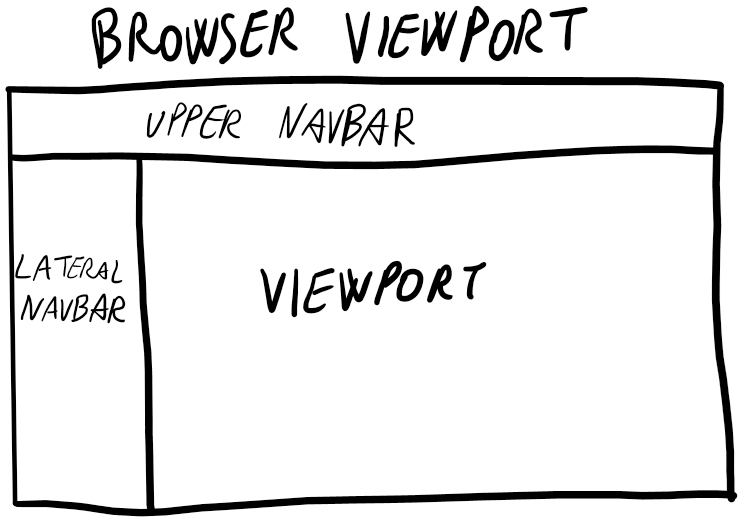
\includegraphics[width=0.5\linewidth]{Images/Browser_viewport.png}
    \caption{Browser viewport}
    \label{fig:viewport}
\end{figure}

\begin{figure}
    \centering
    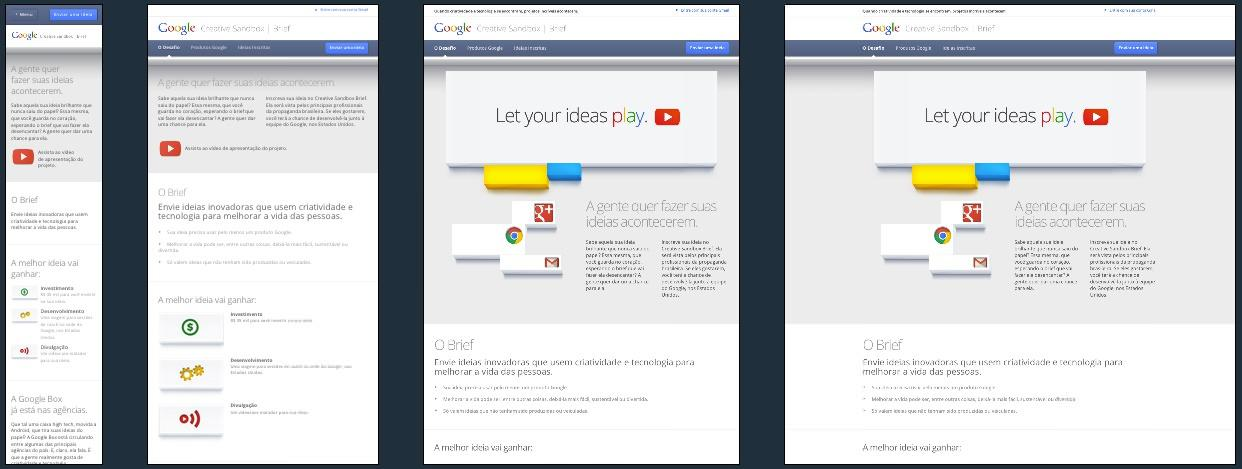
\includegraphics[width=\linewidth]{Images/RWD_example.jpg}
    \caption{Example of Responsive Web Design}
    \label{fig:rwd_example}
\end{figure}

\chapter{Media Queries: Adapting to the Device}

Media Queries are a CSS3 feature that significantly extends the concept of media types found in CSS2. Instead of just targeting a broad device category like \texttt{print} or \texttt{screen}, Media Queries allow styles to be applied based on the specific capabilities and characteristics of a device. This enables developers to create highly tailored experiences by testing features like viewport width, device resolution, and screen orientation.

\section{Syntax and Implementation}

A media query consists of a media type and one or more expressions that check for specific media features. If the conditions are met, the CSS rules within the query are applied. \\

The general syntax for the \texttt{@media} at-rule is:

\begin{lstlisting}[caption={@media at-rule general syntax}]
    @media not|only mediatype and (expressions) { ... }
\end{lstlisting}

Examples of \texttt{@media} at-rule are:

\begin{lstlisting}[caption={@media at-rule examples}]
    @media all and (min-width: 1024px) and (max-width:1280px) {/*** CSS-Code; ***/}

    /* Portrait*/
    @media only screen
    and (min-device-width: 414px)
    and (max-device-width: 736px)
    and (-webkit-min-device-pixel-ratio: 3)
    and (orientation: portrait) {
        /*** CSS-Code; ***/
    }
    
    /* Landscape*/
    @media only screen
    and (min-device-width: 414px)
    and (max-device-width: 736px)
    and (-webkit-min-device-pixel-ratio: 3)
    and (orientation: landscape) {
        /*** CSS-Code; ***/
    }
\end{lstlisting}

There are two primary ways to implement media queries:

\begin{enumerate}
    \item \textbf{Within a single stylesheet:} You can include multiple \texttt{@media} rules directly in your main CSS file. This is the most common approach.
    
    \item \textbf{Linking separate stylesheets:} You can create different CSS files for different media types and link them in your HTML using the \texttt{<link>} tag's \texttt{media} attribute.
\end{enumerate}

\subsection{Primary Media Types}

\begin{table}[htbp]
    \centering
    \begin{tabular}{|l|l|}
    \hline
    \textbf{Media Type} & \textbf{Description} \\
    \hline
    \texttt{all} & Used for all media type devices. \\
    \hline
    \texttt{print} & Used for printers, allowing for printer-friendly page layouts. \\
    \hline
    \texttt{screen} & Used for computer screens, tablets, and smart-phones. \\
    \hline
    \texttt{speech} & Used for screen readers that read the page content aloud. \\
    \hline
    \end{tabular}
    \caption{Primary Media Types}
\end{table}

\subsection{Common Media Features}

\begin{table}[htbp]
    \centering
    \begin{tabular}{|l|l|}
    \hline
    \textbf{Media Feature} & \textbf{Description} \\
    \hline
    \texttt{width} & The width of the viewport. \\
    \hline
    \texttt{height} & The height of the viewport. \\
    \hline
    \texttt{device-width} & The width of the device's screen. \\
    \hline
    \texttt{device-height} & The height of the device's screen. \\
    \hline
    \texttt{orientation} & The orientation of the viewport (either \texttt{portrait} or \texttt{landscape}). \\
    \hline
    \texttt{resolution} & The resolution of the output device (in \texttt{dpi} or \texttt{dppx}). \\
    \hline
    \end{tabular}
    \caption{Common Media Features}
\end{table}

\section{Understanding Device Pixel Ratio (DPR)}

Device Pixel Ratio (DPR) is the ratio between the physical pixels on a hardware screen and the logical (CSS) pixels used for layout. This ratio is crucial for ensuring that images and graphics appear sharp on high-resolution displays, such as Apple's Retina screens. \\

The formula for DPR is: \texttt{DPR = Physical Pixels / CSS Pixels} \\

DPR is important because ignoring it can lead to blurry visuals. For example, if a 100px by 100px image is displayed on a device with a DPR of 2.0, each logical pixel is stretched to fit a 2x2 grid of physical pixels. This stretching causes the image to appear pixelated and less crisp. Imagine trying to create a sharp photograph using only four large Lego bricks; the result is blocky and indistinct. This is analogous to how a low-resolution image appears on a high-DPR screen. \\

To target devices with different DPRs, you can use media queries to serve higher-resolution assets. There are two primary CSS methods for this:

\begin{enumerate}
    \item \textbf{The standard} \texttt{\textbf{resolution}} \textbf{feature:} This is the modern, standardized approach. The \texttt{dppx} unit stands for "dots per px".
    \item \textbf{The non-standard} \texttt{\textbf{-webkit-min-device-pixel-ratio}} \textbf{feature:} This prefixed version was introduced by the WebKit rendering engine and is still necessary for ensuring compatibility with some older WebKit-based browsers.
\end{enumerate}

After querying a device's properties to determine which styles to apply, the next step is to use robust layout systems that can effectively organize content based on that information.

\chapter{Modern CSS Layout Techniques}

Early web layouts often relied on HTML \texttt{<table>} elements to structure page content. This technique is now considered deprecated because it is semantically incorrect and highly inflexible, making it unsuitable for responsive design. Modern CSS provides dedicated layout modules that offer powerful solutions for creating robust and adaptive designs. The two most prominent techniques are CSS Grid Layout and the Flexible Box Layout (Flexbox). It's critical to understand their distinct purposes: \textbf{Flexbox} is a one-dimensional system, ideal for laying out items in a single row or column, such as navigation bars or form elements. \textbf{Grid} is a two-dimensional system, designed to control layout in both rows and columns simultaneously, making it perfect for overall page structure.

\section{The Grid View System}

\begin{figure}
    \centering
    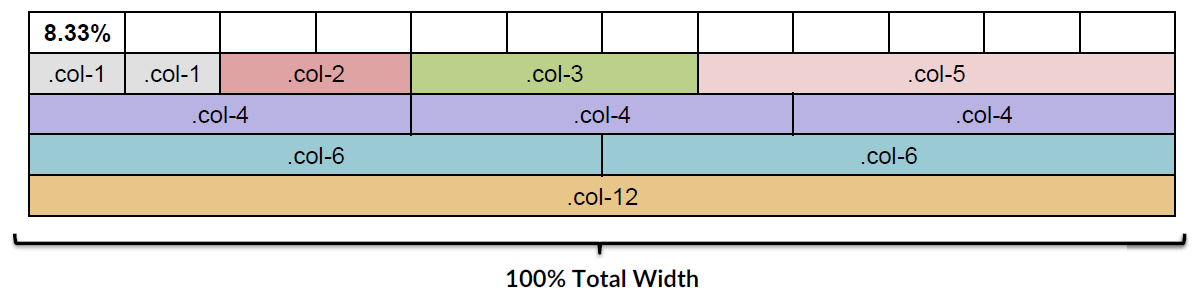
\includegraphics[width=\linewidth]{Images/Gridview.png}
    \caption{Grid view system}
    \label{fig:grid_view_system}
\end{figure}

A common conceptual approach to layout, popularized by frameworks like Bootstrap, involves dividing the page into a set number of columns, typically 12. This system helps developers place elements on the page by assigning them CSS classes that correspond to a specific number of columns the element should occupy (See figure ~\ref{fig:grid_view_system}). \\

Its primary purpose is to simplify the creation of organized, column-based layouts. Elements are arranged in rows, and their widths are defined by the number of grid columns they span. This system has a built-in responsive behavior: if the sum of the column classes in a single row exceeds the total available (e.g., 12), the overflowing element automatically reflows onto the next line. This allows the layout to adapt fluidly to different viewport sizes. It is important to differentiate this framework-based approach from the native \textbf{CSS Grid Layout} module, which is a more powerful, built-in browser feature for two-dimensional layouts that does not rely on predefined classes.

\section{Flexbox: The Flexible Box Layout Model}

\begin{figure}[htbp]
    \centering
    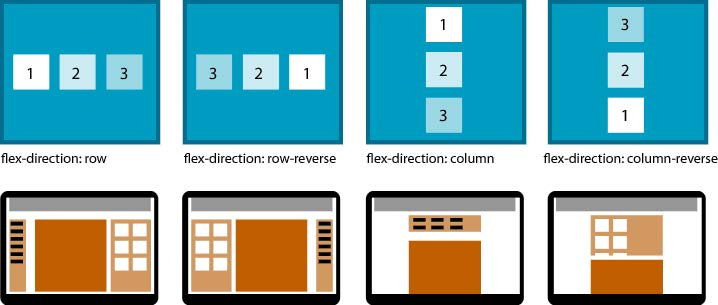
\includegraphics[width=\linewidth]{Images/Flexbox.jpg}
    \caption{Flexible box layout}
    \label{fig:flexbox}
\end{figure}

Flexbox, or the Flexible Box Layout model, is a one-dimensional layout model designed to provide a more efficient way to distribute space and align items within a container. It excels at managing the layout of components and small-scale structures within a larger design. \\


The Flexbox model is built on two core components:

\begin{itemize}
    \item \textbf{Flex Container:} The parent element that holds the flex items. A flex container is created by setting its \texttt{display} property to \texttt{flex} or \texttt{inline-flex}.
    \item \textbf{Flex Items:} The direct children of the flex container. These items are laid out and aligned according to the rules set on the container.
\end{itemize}

Flexbox operates along two primary axes, which define the direction of the layout:

\begin{itemize}
    \item \textbf{Main Axis:} The primary axis along which flex items are laid out. The \texttt{flex-direction} property defines this axis, which can be horizontal (\texttt{row}) or vertical (\texttt{column}).
    \item \textbf{Cross Axis:} The axis that runs perpendicular to the main axis.
\end{itemize}

\newpage

\subsection{Properties for the Flex Container}

The following properties are applied to the parent element (the flex container) to control the layout of its children.

\begin{table}[h]
    \centering
    \begin{tabularx}{\linewidth}{|l|X|X|}
        \hline
        \textbf{Property} & \textbf{Description} & \textbf{Common Values} \\
        \hline
        \texttt{display} & Defines the element as a flex container. & \texttt{flex}, \texttt{inline-flex} \\
        \hline
        \texttt{flex-direction} & Establishes the main axis, defining the direction items are placed. & \texttt{row}, \texttt{row-reverse}, \texttt{column}, \texttt{column-reverse} \\
        \hline
        
        \texttt{flex-wrap} & Controls whether flex items wrap onto a new line if they overflow. (See figures ~\ref{fig:row_overflow} and ~\ref{fig:column_overflow}) &
        \texttt{nowrap}, \texttt{wrap}, \texttt{wrap-reverse}. (\texttt{nowrap} forces all the child elements to be in the same line. In case the child elements overflow the container they might become inaccessible to the user so, in case we decide to use the \texttt{nowrap} option, it is advisable to use the \texttt{overflow: scroll} option referring to the main axis of the flexbox.) \\
        \hline
        
        \texttt{flex-flow} & A shorthand for \texttt{flex-direction} and \texttt{flex-wrap}. & \texttt{row wrap}, \texttt{column nowrap} \\
        \hline
        \texttt{justify-content} & Aligns flex items along the main axis, distributing extra space. & \texttt{flex-start}, \texttt{flex-end}, \texttt{center}, \texttt{space-between}, \texttt{space-around}, \texttt{space-evenly} \\
        \hline
        \texttt{align-items} & Aligns flex items along the cross axis. & \texttt{stretch}, \texttt{flex-start}, \texttt{flex-end}, \texttt{center}, \texttt{baseline} \\
        \hline
        \texttt{align-content} & Aligns a container's lines when there is extra space on the cross axis, similar to how \texttt{justify-content} aligns items on the main axis. Only affects multi-line containers (\texttt{flex-wrap: wrap}). & \texttt{flex-start}, \texttt{flex-end}, \texttt{center}, \texttt{space-between}, \texttt{space-around}, \texttt{stretch} \\
        \hline
    \end{tabularx}
    \caption{Properties for the Flex Container}
\end{table}

\begin{figure}
    \centering
    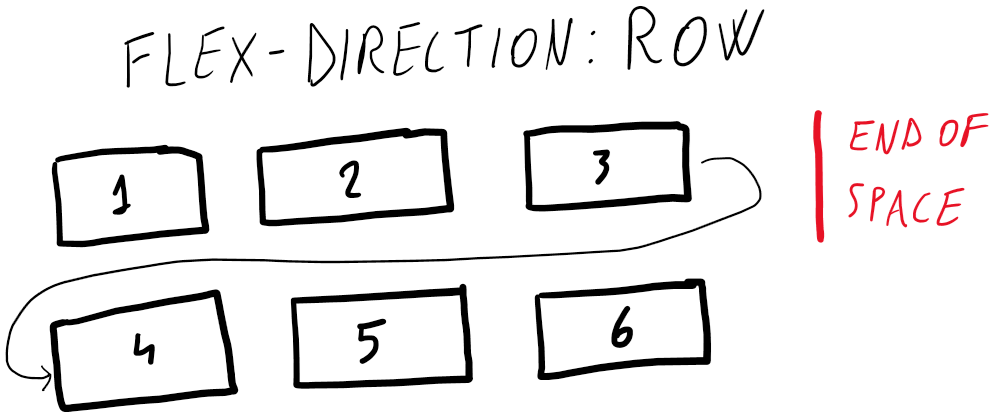
\includegraphics[width=\linewidth]{Images/Flex_direction_row_overflow.png}
    \caption{Flexbox row overflow with wrap}
    \label{fig:row_overflow}
\end{figure}

\begin{figure}
    \centering
    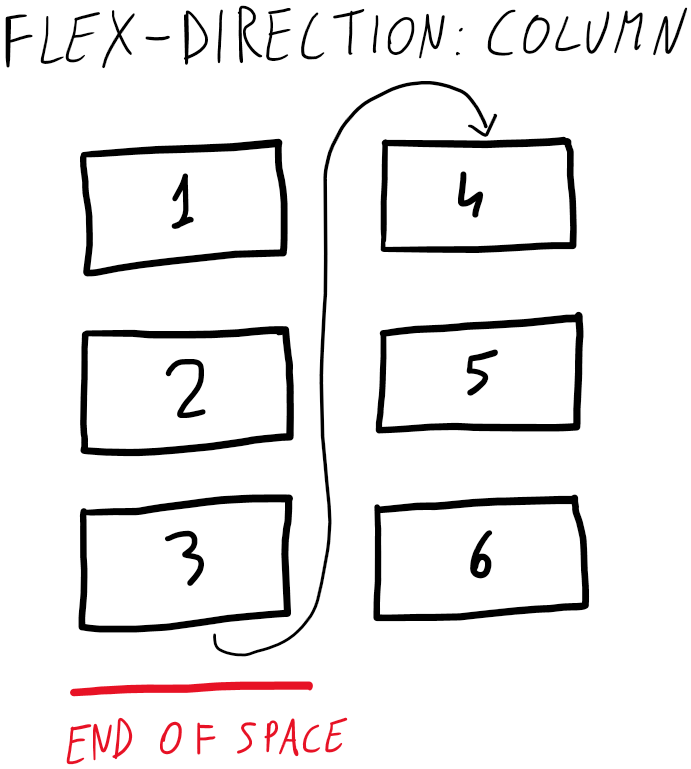
\includegraphics[width=0.5\linewidth]{Images/Flex_direction_column_overflow.png}
    \caption{Flexbox column overflow with wrap}
    \label{fig:column_overflow}
\end{figure}

\newpage

\subsection{Properties for Flex Items}

These properties are applied to the child elements (the flex items) to control their individual behavior within the container.

\begin{table}[h]
    \centering
    \begin{tabularx}{\linewidth}{|l|X|X|}
        \hline
        \textbf{Property} & \textbf{Description} & \textbf{Common Values} \\
        \hline
        \texttt{order} & Controls the order in which items appear in the container. & \texttt{<integer>} (e.g., -1, 0, 1) \\
        \hline
        \texttt{flex-grow} & Defines the ability of an item to grow, taking up available space. & \texttt{<number>} (e.g., 0, 1, 2) \\
        \hline
        \texttt{flex-shrink} & Defines the ability of an item to shrink if there is not enough space. & \texttt{<number>} (e.g., 0, 1, 2) \\
        \hline
        \texttt{flex-basis} & Defines the default size of an item before remaining space is distributed. & \texttt{<length>} (e.g., 200px, 50\%, auto) \\
        \hline
        \texttt{flex} & A shorthand for \texttt{flex-grow}, \texttt{flex-shrink}, and \texttt{flex-basis}. & \texttt{0 1 auto} (default), \texttt{1}, \texttt{none} \\
        \hline
        \texttt{align-self} & Overrides the default alignment set by \texttt{align-items} for an individual item. & \texttt{auto}, \texttt{flex-start}, \texttt{flex-end}, \texttt{center}, \texttt{stretch}, \texttt{baseline} \\
        \hline
    \end{tabularx}
    \caption{Properties for Flex Items}
\end{table}

Beyond static layouts, CSS also provides powerful tools for creating dynamic visual effects, such as animations.

\chapter{Dynamic Visuals with CSS Animations}

\begin{figure}[htbp]
    \centering
    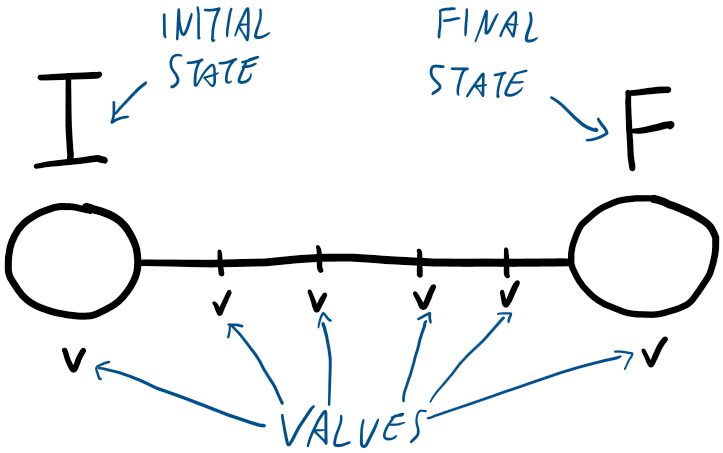
\includegraphics[width=0.5\linewidth]{Images/Animation.png}
    \caption{CSS animation divided in steps}
    \label{fig:animation}
\end{figure}

CSS Animations are a feature that allows the transformation of an element's properties from an initial state to a final state over a specified duration. This makes it possible to create complex, multi-step visual effects like movement, color changes, and fading without relying on JavaScript. \\

The core of a CSS animation is the \texttt{@keyframes} at-rule. This rule is used to define the animation's intermediate steps, or "keyframes", as percentages of the overall duration (See figure ~\ref{fig:animation}). For simple transitions between a start and end state, the keywords \texttt{from} (equivalent to 0\%) and \texttt{to} (equivalent to 100\%) can be used instead of percentages. \\

A conceptual \texttt{@keyframes} rule looks like this:

\begin{lstlisting}
@keyframes myAnimation {
  from { background-color: red; }
  to   { background-color: yellow; }
}
\end{lstlisting}

Once an animation is defined with \texttt{@keyframes}, it can be applied to an element using several key properties:

\begin{itemize}
    \item \texttt{\textbf{animation-name}}: Specifies the name of the \texttt{@keyframes} rule to apply.
    \item \texttt{\textbf{animation-duration}}: Sets how long the animation should take to complete one cycle.
    \item \texttt{\textbf{animation-delay}}: Specifies a delay before the animation starts.
\end{itemize}

Understanding how CSS rules are defined is one part of the equation; the other is understanding the software that interprets and renders them.

\chapter{A Note on Rendering Engines and Prefixes}

A browser's \textbf{rendering engine} is the core software component responsible for interpreting HTML, CSS, and other web content to calculate the layout and render the visual representation of a web page. Different browsers may use different rendering engines. \\

\textbf{WebKit} is a prominent open-source rendering engine initially created by Apple. It powers browsers like Apple's Safari and was formerly used by Google Chrome. Rendering engines are where new or experimental CSS features are often first implemented. \\

To implement these non-standard or experimental features without conflicting with existing standards, rendering engines use \textbf{vendor-specific prefixes}. A common example is the \texttt{-webkit-} prefix, used by the WebKit engine. For instance, the \texttt{-webkit-device-pixel-ratio} media feature was a non-standard feature introduced by WebKit to handle high-DPR displays before a standardized equivalent was widely adopted. \\

While these prefixes are sometimes necessary to ensure broad compatibility with older browsers, developers should prioritize using standard, unprefixed CSS features (like the \texttt{resolution} media feature) whenever possible. Standard features are supported across all modern rendering engines, leading to more maintainable and future-proof code.


\end{document}
